\titleformat{\chapter}[display]
{\normalfont\huge\bfseries}{Capítulo \thechapter}{0.5em}{\huge}
\titlespacing*{\chapter}{0pt}{-1.25cm}{25pt}
\chapter{Introducción}
\section{Concepto de arritmia}
Las enfermedades cardiovasculares son la primera causa de muerte en el mundo y una de las causas más comunes de estas enfermedades son las arritmias.

Una arritmia cardiaca es una alteración en el ritmo normal del corazón. Si se produce una arritmia, el corazón puede latir demasiado rápido, demasiado lento o de manera irregular. Esto puede provocar síntomas como palpitaciones, mareos, falta de aire e incluso desmayos y estas pueden llegar a ser mortales.

Los cardiólogos utilizan dispositivos como un \textit{Holter} para generar electrocardiogramas (ECG), que son diagramas que representan los latidos del corazón y con ellos son capaces de analizarlos y encontrar anomalías cardiacas.

Entre esas anomalías están las contracciones prematuras del corazón, un tipo de arritmia que este proyecto se encargará de detectar. 

\begin{figure}[h!]
	\centering
	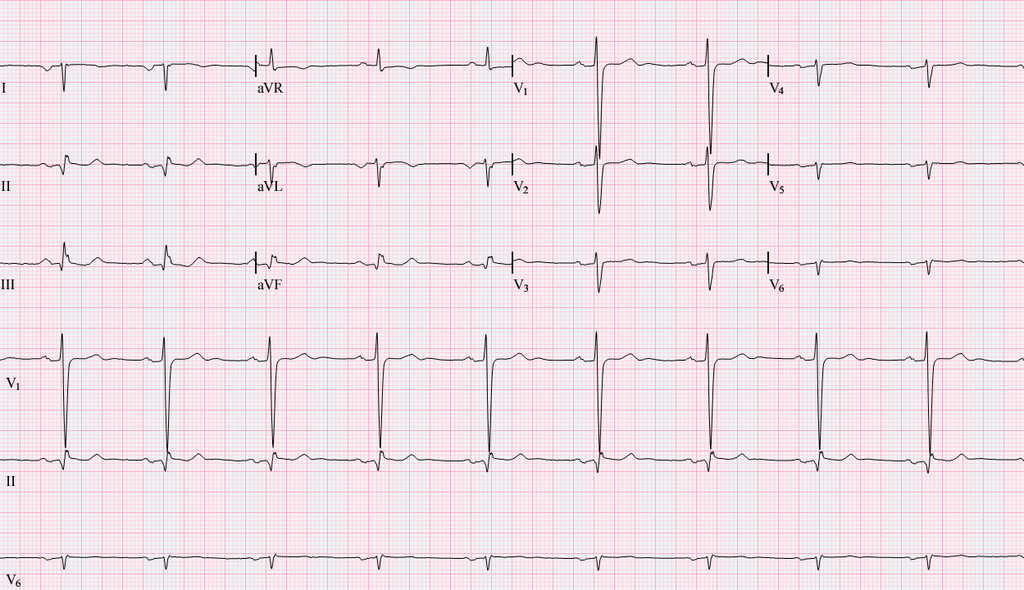
\includegraphics[width=0.7\textwidth]{./Images/img_introduccion/electrocardiograma.png}
	\caption{Imagen de varios electrocardiogramas recopilados por un \textit{Holter}.}
	\label{fig:electrocardiogramas}
\end{figure}

\section{Algoritmo de detección}
El algoritmo de detección de arritmias que sigue este proyecto se basa en la detección de 
los picos QRS producidos en el electrocardiograma.

Un pico QRS, como se muestra en la \Cref{fig:complejoQRS} en un electrocardiograma es causado por la contracción del ventrículo al bombear la sangre por las arterias. Este es el impulso eléctrico más fuerte que el corazón produce en cada latido. En este proyecto utilizaremos estos picos para comparar la distancia entre ellos y poder determinar si se ha producido una arritmia. 

\begin{figure}[h]
	\centering
	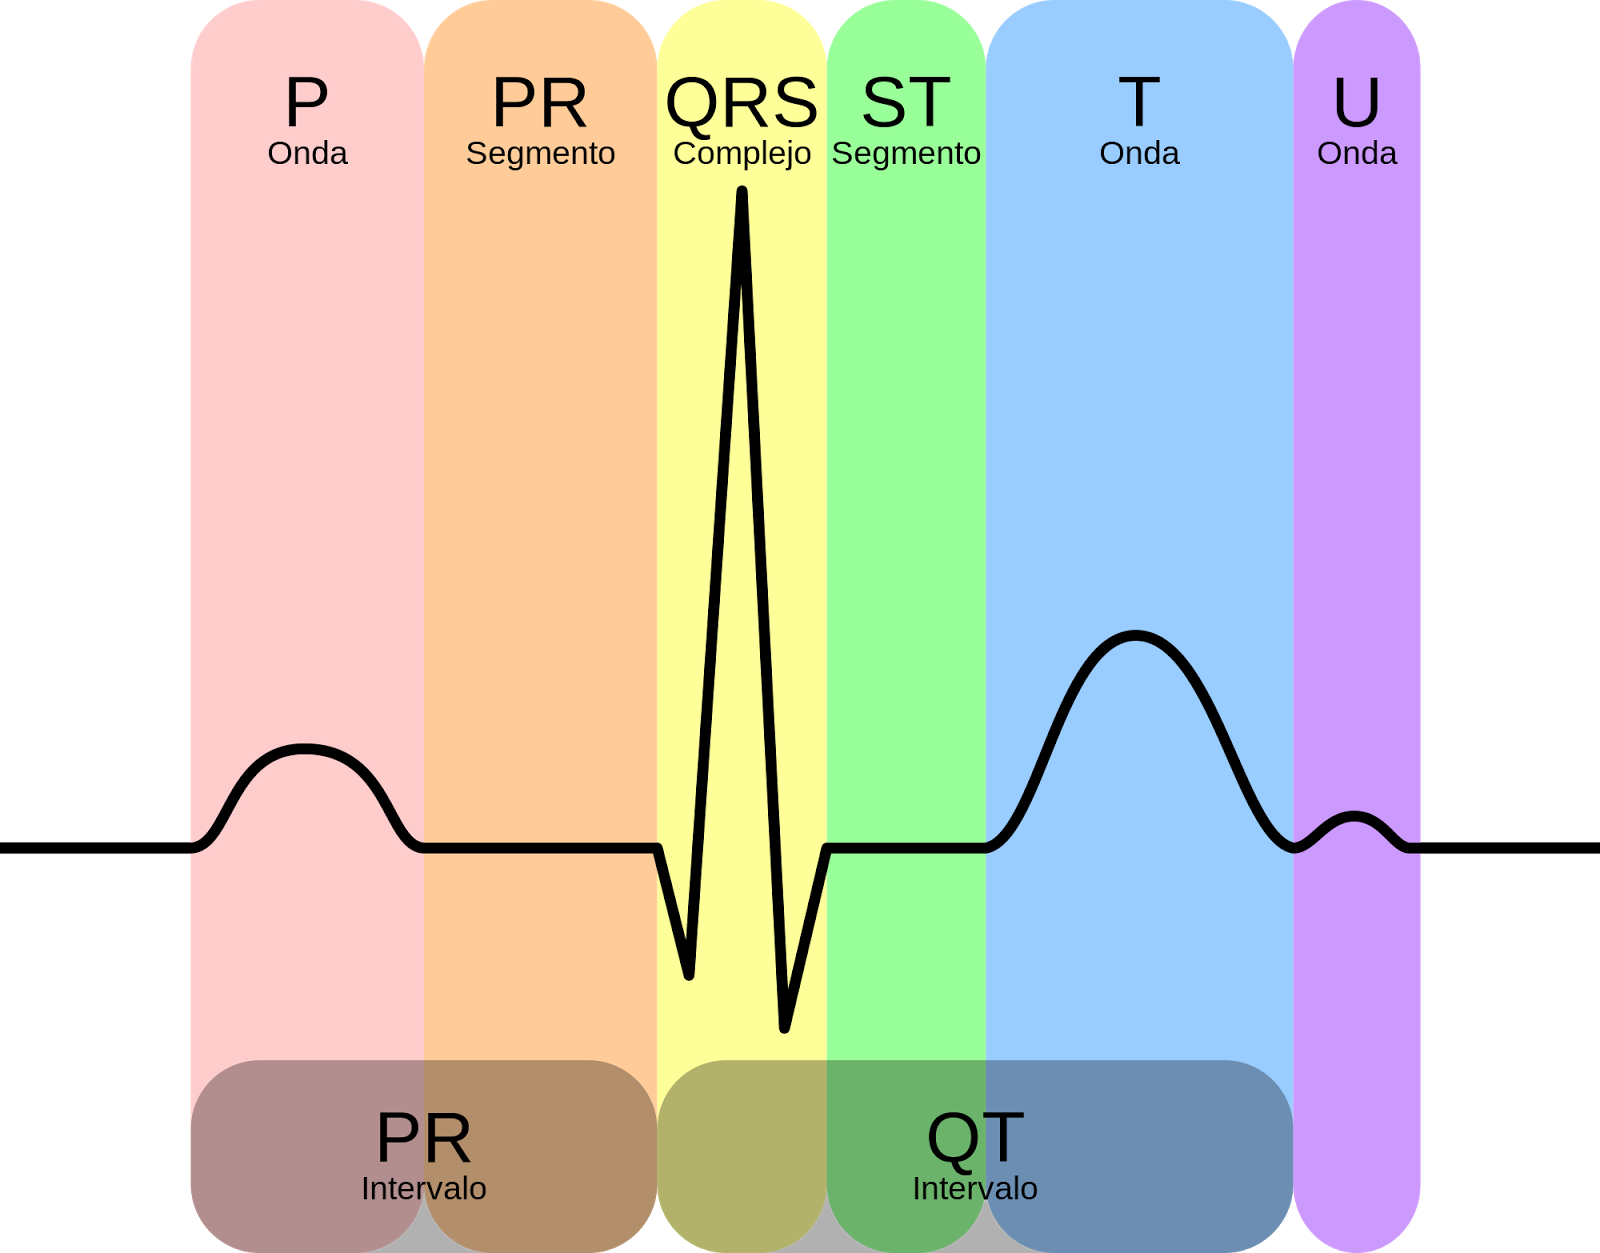
\includegraphics[width=0.4\textwidth]{./Images/img_introduccion/complejoQRS.png}
	\caption[Complejo QRS]{Complejo QRS \cite{desai2021low}}
	\label{fig:complejoQRS}
\end{figure}

\subsection{Filtrado}
Como se puede observar en la \Cref{fig:102filtradoysinfiltrar} es conveniente hacer un filtrado de las tiras de ritmo para poder detectar mejor los picos QRS, ya que el filtrado centra la onda en el valor 0 y evita fallos en el algoritmo de detección de picos del que se hablará más adelante. 

En la creación del proyecto se ha intentado no filtrar la onda para comprobar si se obtienen mejores resultados que sin dicho filtrado, pero no se ha dado el caso por las irregularidades de la misma.

\begin{figure}[h!]
	\centering
	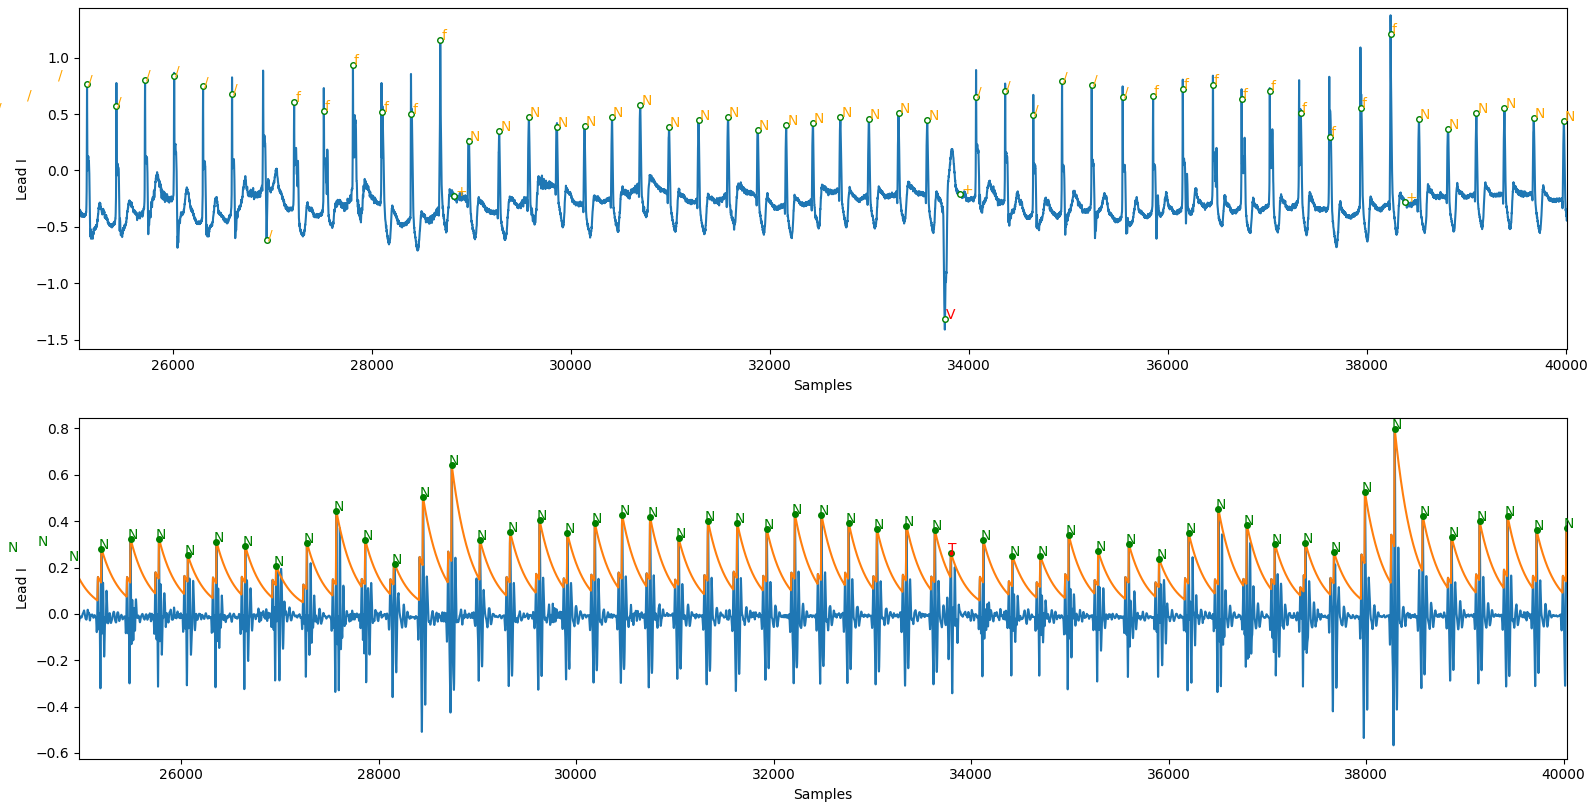
\includegraphics[width=0.99\textwidth]{./Images/img_introduccion/102filtrado_y_sin_filtrar.png}
	\caption{Ejemplo de electrocardiograma original y filtrado de paciente 102 (Elaboración propia)}
	\label{fig:102filtradoysinfiltrar}
\end{figure}

\section{Datos de referencia}
Los datos de referencia para probar el algoritmo han sido obtenidos de un estudio realizado en el Instituto de Tecnología de Massachusetts (MIT) en el que se han realizado pruebas de media hora a varios pacientes con edades diversas y algunos de ellos llevaban implantado un marcapasos.

Los datos consisten en electrocardiogramas que previamente han sido analizados por cardiólogos y cuyas anotaciones indican cuando un paciente ha padecido una arritmia, cuando el ritmo es normal y cuando se ha producido un fallo en la lectura de la señal. También se muestra información menos relevante para nuestro 
estudio como cuando se ha producido un error en la lectura de la señal y la activación del marcapasos\footnote{\textbf{Marcapasos}: Dispositivo que se implanta en el corazón que actúa cuando el corazón no bombea la sangre lo suficientemente fuerte, es decir que el pico QRS no es tan prominente
y se necesita la ayuda de dicho dispositivo para proporcionar el impulso eléctrico necesario}.

\begin{figure}[h]
	\centering
	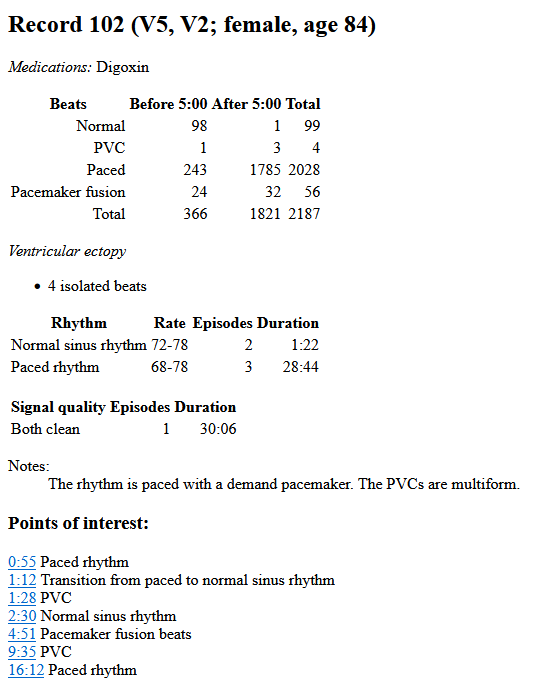
\includegraphics[width=0.6\textwidth]{./Images/img_introduccion/Paciente_pruebas_MIT.png}
	\caption{Ejemplo con paciente 102 \cite{mitdb}}
	\label{fig:Paciente_pruebas_MIT}
\end{figure}

\section{Utilización de las FPGAs}
Este programa ha sido pensado para ejecutarse en un dispositivo pequeño, poco pesado y portable, es por ello, que es conveniente ejecutarlo en una FPGA, esto de debe a que una FPGA con una placa pequeña tiene el hardware suficiente para poder llegar a ejecutar este programa y por ello pueden
ser llevados con facilidad, además el consumo producido por una FPGA al ejecutar el algoritmo es bastante bajo como se comprobará posteriormente.

Para este proyecto se usará la FPGA Artix-7 en la placa Basys3 para probar el funcionamiento del algoritmo. Aunque se debe considerar, según la cantidad de datos introducidos, que en este caso sería la longitud de la señal según el tiempo transcurrido, utilizar una FPGA cuyo hardware pueda soportar dicha cantidad de datos.


\section{Objetivos del proyecto}

El objetivo principal del proyecto es crear un algoritmo que detecte arritmias en los pacientes y que dicho algoritmo sea capaz de ejecutarse en un dispositivo portable 
que tenga un bajo consumo y que funcione a tiempo real.
Para conseguir el objetivo principal es necesario alcanzar una serie de objetivos que son los siguientes:
\begin{enumerate}
	\item Averiguar que son las arritmias, como se producen, que arritmias podría detectar el programa y que patrón siguen la mayoría de ellas.

	\item La creación de un algoritmo en software que sea capaz de leer y filtrar la señal original de los pacientes de la base de datos, la realización de
	un algoritmo que se encargue de detectar los picos donde se produce la contracción ventricular según aparecen en la señal filtrada, por último la creación 
	de un algoritmo encargado de detectar las arritmias según el patrón hallado en el objetivo anterior.
	
	\item La replicación del programa en hardware según el prototipo creado anteriormente en software. Utilizando el hardware necesario para que el algoritmo funcione en una FPGA 
	y el hardware necesario para poder hacer pruebas en simulación y sobre la placa.  

	\item La observación de los resultados experimentales de la cantidad de recursos hardware empleados, el consumo causado por el algoritmo y el tiempo que tarda en 
	llevarse a cabo adecuándose a la llegada de la señal del paciente. Dichos resultados experimentales deberían tener una coherencia con lo que se buscaba en el objetivo principal.
\end{enumerate}

\section{Análisis y optimización del algoritmo}
El algoritmo se centra en tres funciones principales.
\begin{enumerate}
	\item Filtrado de la señal original: Lo que hace que la señal sea más fácil de procesar para encontrar los picos QRS.
	 Esto se realiza multiplicando los valores de la señal original por los valores de filtrado almacenados en una memoria.
	\item Detección de picos sobre la señal filtrada: Se analiza cada valor de la señal filtrada y si dicho valor es mayor que
	 sus anteriores, se considera un posible pico, si después de 72 valores se mantiene como el valor más alto, entonces ese valor
	 se considera un pico QRS.
	\item Detección de arritmias comparando la posición de los picos: Una vez obtenidos los picos QRS se calcula la distancia
	 del pico actual con el pico anterior y dependiendo de las distancias anteriores, se calcula si hay una arritmia.
\end{enumerate}


\section{Implementación en la FPGA}
Para implementar el código en la FPGA se implementarán varios módulos que por lo general, tratan de replicar las funcionalidades que realiza
el algoritmo de software y se convertirán en la parte más importante de dicho programa.  

Los módulos más importantes son.

	\begin{enumerate}
		\item Módulo de filtrado: Se guardan los valores del filtrado en un módulo de memoria ROM y los valores de la señal original en una memoria RAM 
		cuando los valores de la RAM son multiplicados, se escribe en la RAM y se pasan los valores al siguiente módulo principal.
		\item Módulo de detección de picos sobre la señal filtrada: Se implementa una máquina de estados que analiza cada valor de
		 la señal filtrada y calcula si es un posible pico, o un pico QRS. Como los valores de la señal son números reales, se implementan varios módulos para
		 poder operar con los valores de la señal. 
		\item Módulo de detección de arritmias: Se implementa una máquina de estados con el que recibiendo un pico QRS como entrada, sea capaz de almacenar las
		 distancias más recientes, calcular según la diferencia de estas distancias, si se ha producido una arritmia y mostrar como salida un flag indicándolo.
	\end{enumerate}
	
	Además de estos módulos se debe de crear un módulo que los acompase y un testbench para probar el funcionamiento del programa en la simulación.

\section{Organización de la memoria}
Para empezar se verá como se ha realizado el prototipado del algoritmo en software. Se indicarán las librerías usadas para la recopilación de datos,
El tipo de filtrado que se ha usado para el filtro de la señal original, El algoritmo de la detección de picos QRS y las metodologías que se han seguido,
el algoritmo de detección de arritmias y el algoritmo de pruebas seguido para probar el algoritmo original en su totalidad y para poder sacar estadísticas 
de las pruebas realizadas.

Para continuar se hablará de los distintos módulos creados para la implementación hardware. Se especificarán los módulos para las operaciones en punto
flotante, los módulos para las memorias utilizadas. Se profundizará sobre los módulos principales basados en el prototipo del software y por último la creación 
del módulo principal y el testbench utilizado.

Seguidamente se mostrarán los resultados experimentales obtenidos, la FPGA utilizado, el análisis de síntesis, el análisis de timing y el consumo.

Finalmente se dará una conclusión de la realización de este proyecto y unos trabajos futuros por si se desea ampliar el proyecto.
